\documentclass[11pt,a4paper]{article}
\usepackage[left=2.5cm,right=2.5cm,top=3cm,bottom=3.5cm]{geometry}
\usepackage[ngerman]{babel}
\usepackage[utf8]{inputenc}
\usepackage{graphicx}
\usepackage{amsfonts} 
\usepackage{svg}
\usepackage{amsmath}
\begin{document}
 
 \begin{center}
  {\scshape\LARGE Grundpraktikum I \par}
  \vspace{1cm}
  {\scshape\Large Versuchsprotokoll\par}
  \vspace{1.5cm}
  {\huge\bfseries Isentropenindex\par}
  \vspace{2cm}
     {\large \itshape{Clemens Schumann, Tassilo Scheffler}\/ \par}
  \vspace{0.5cm}
  {clemensrubenschumann@googlemail.com, \\ tassilo@glief.de}
  \vfill
  betreut von\par
  \textsc{Larissa Melischek}
  \vfill
  {\Large 10.03.2018}
 
 \end{center}
 
 \thispagestyle{empty}
 
 \newpage
 \setcounter{page}{1}
 \tableofcontents
 \newpage
 \section{\underline{Physikalische Grundlagen}}
 \subsection{Innere Energie und W\"armekapazit\"at}
 In einem abgeschlossenem System bleibt der Gesamtbetrag der Energie konstant.
 Innerhalb des Systems k\"onnenn sich die verschiedenen Energien ineinander umwandeln
 (1. Hauptsatz der Thermodynamik). Dabei sind die verschiedenen Energien die
 kinetische Energie $E_{kin}$, die potentielle Energie $E_{pot}$ und die innere Energie U
 des Systems. Diese innere Energie beschreibt die gesamte thermische Energie bzw.\ die
 gesamte kinetische und potentielle Energie des Systems. Die \"Anderung $dU$
 l\"asst sich mit der \"Anderung $dW$ der Arbeit und dem W\"arme\"ubertrag $dQ$
 bestimmen.
 \begin{align}
     \label{f1}
     dU=dQ+dW
 \end{align}
 Mithilfe des W\"arme\"ubertrags und der Temperatur\"anderung $dT$ l\"asst sich die
 W\"armekapazit\"at $C$ definieren:
 \begin{align}
     \label{f2}
     C=\frac{dQ}{dT}
 \end{align}
 Dies ist von der Masse $m$ ab\"angig, weswegen man die spezifische W\"armekapazit\"at
 \begin{align}
     \label{f3}
     c=\frac{C}{m}
 \end{align}
 definiert. M\"ochte man stattdessen eine Unabh\"angigkeit von der Stoffmenge M, so ist
 \begin{align}
     \label{f4}
     C_{m}=\frac{c}{n}
 \end{align}
 als molare W\"armekapazit\"at definiert, wobei n die Molanzahl ist. Die
 W\"armekapazit\"at ist stoffabh\"angig und wird in $\frac{Joule}{Kelvin}$ angegeben.
 \subsection{Gase}
 F\"ur ideale Gase (bestehend aus punktf\"ormigen isotropen Kugeln, welche nur
 elastische St\"o{\ss}e untereinander betreiben) gilt immer eine Zustandsgleichung.
 \begin{align}
     \label{f5}
     \frac{pV}{T}=konstant=n \cdot R=N \cdot k_{B}
 \end{align}
 Nach der kinetischen Gastheorie definiert man den Druck des Gases als Folge der
 St\"o{\ss}e, die die Gasmolek\"ule auf die Gef\"a{\ss}wand aus\"uben. \\
 Nun k\"onnen die Zust\"ande eines Gases verschieden ge\"andert werden. Als erstes sei
 die isochore Zustands\"anderung (v=konstant) genannt. F\"ur diese kann nun
 \begin{align}
     \label{f6}
     dU=C_{V}dT
 \end{align}
 \begin{align}
     \label{f7}
     C_{V}=N \frac{f}{2} k_{B}
 \end{align}
 hergeleitet werden. Die Freiheitsgrade sind die Anzahl der unabh\"angigen Parameter,
 die ben\"otigt werden, um ein System zu beschreiben. Es gibt 3 Freiheitsgrade der
 Translation, 2 der Rotation und 2 der Schwingung eines Molek\"uls bzw.\ Systems. \\
 Als zweites sei hier die isobare Zustands\"anderung eines Gases (p=konstant) genannt.
 Hierf\"ur wird \"ahnlich definiert:
 \begin{align}
     \label{f8}
     Vdp = C_{p}dT
 \end{align}
 und
 \begin{align}
     \label{f9}
     C_{p}=N\left(\frac{f}{2}+1\right)k_{B}
 \end{align}
 In einer dritten, sogenannten adiabatischen (isentropen) zustands\"anderung l\"asst
 sich das vorige zusammenbringen. Denn hierbei darf nur kein W\"armeaustausch mit der
 Umgebung stattfinden ($dQ=0$) bzw.\ die Entropie muss gleichbleibend sein.
 Demenstprechend finden auch nur reversible Prozesse statt. Damit wird aus~\eqref{f6}
 und~\eqref{f1}:
 \begin{align}
     \label{f10}
     dU=dW=-pdV=C_{V}dT
 \end{align}
 Mithilfe von~\eqref{f8} und~\eqref{f10}, indem man jeweils $dT$ isoliert, er\"alt man
 \begin{align}
     \label{f11}
     \frac{c_{p}}{c_{V}}Vdp=-pdV \leftrightarrow \frac{1}{p}dp=-\frac{\kappa}{V}dV
 \end{align}
 wobei
 \begin{align}
     \label{f12}
     \kappa = \frac{c_{p}}{c_{V}} 
 \end{align}
 benutzt wurde. Integrieren von $p_{1},V_{1} \rightarrow p_{2},V_{2}$ und exponenzieren
 von~\eqref{f11} ergibt
 \begin{align}
     \label{f13}
     \frac{p_{2}}{p_{1}} = {\left(\frac{V_{1}}{V_{2}}\right)}^{\kappa} \rightarrow
     p \cdot {V}^{\kappa} = konst.\
 \end{align}
 Mit~\eqref{f5} wird dies zu
 \begin{align}
     \label{f14}
     T\cdot{V}^{\kappa-1}=konst.\
 \end{align}
 und
 \begin{align}
     \label{f15}
     {p}^{1-\kappa}{T}^{\kappa}=konst.\
 \end{align}
 Die Gleichungen~\eqref{f13},\eqref{f14} und~\eqref{f15} werden Poisson-Gleichungen
 oder auch Adiabatengleichungen genannt. Der Isentropenindex $\kappa$ kann experimentell
 ermittelt werden. Dazu bieten sich mehrere Methoden an. Im Rahmen des Grundpraktikums
 werden die Methoden nach Clement-Desormes und nach Flammersfeld-R\"uchart verwendet. 
 \newpage
 \subsection{Methode nach Clement-Desormes}
 Bei dieser Methode zur Bestimmung von $\kappa$ wird ein \"Uberdruck in einem
 Glasbeh\"alter erzeugt. Nach dem thermischem Ausgleich auf Zimmertemperatur wird ein
 Entl\"uftungsventil kurzzeitig ge\"offnet, wodurch eine nahezu afiabatische
 Zustands\"anderung erfolgt. Anschlie{\ss}end findet eine isochore Zustands\"anderung
 statt, bis die Zimmertemperatur wieder erreicht ist. \\
  Daher kann für die adiabatische Zustandsänderung (a), bei der das Volumen konstant bleibt, die Poisson-Gleichung (15) benutzt werden. Mithilfe des totalen Differentials ergibt sich
\begin{equation}
    \label{f16}
  (1-\kappa)\frac{dp_{(a)}}{p} + \kappa \frac{dT_{(a)}}{T} = 0
\end{equation}
Aus
\begin{align}
    \label{f17}
  \frac{p}{T} = konst.
\end{align}
und
\begin{equation}
    \label{f18}
  \frac{dp_{(i)}}{T}-p\frac{dT_{(i)}}{T^2}=0
\end{equation}
für die isochore Zustandsänderung ergibt sich nach isolieren von $\frac{dT_{(i)}}{T}$ und einsetzten in~\eqref{f18} mit $dT_{(i)}=-dT_{(a)}$:
\begin{align}
    \label{f19}
    0 & = (1-\kappa)\frac{dp_{(a)}}{p} + \kappa \frac{dp_{(i)}}{p}  \\
  \Leftrightarrow
  \kappa & = \frac{dp_{(a)}}{dp_{(a)}}+dp{(i)} \\
    &\approx \frac{\Delta h_{1}}{\Delta h_{1}-{\Delta}h_{2}}
\end{align}
wobei h die die H\"ohe der Fl\"ussigkeit im Manometer ist.
\subsection{Methode nach Flammersfeld-Rüchert}
Bei dieser Methode wird beispielsweise eine Kugel in eine abgeschlossene Röhre fallen gelassen, in der Überdruck herrscht. Ein Querschlitz ist in der Röhre ungefähr bei der Mitte. Wenn nun die Kugel fallen gelassen wird, so fällt sie unter den Querschlitz und wird dann wieder wegen des Überdrucks zurückgedrückt. Dadurch findet eine Schwingung statt, bei der die Kugel periodisch schwingt. Dementsprechend wirkt die Kraft
\begin{align}
    \label{f20}
  dF&=-Ddx \\
  &=dpS
\end{align}
mit S als Querschnittsfläche, x als Auslenkung und 
\begin{equation}
    \label{f21}
D=m\omega^2
\end{equation}
 als Rückstellkonstante. \\
Hier wird die Adiabatengleichung $pV^\kappa=konst$~\eqref{f13} verwendet. Mithilfe des totalen Differentials ergibt sich:
\begin{equation}
    \label{f22}
  \frac{dp}{p}+\kappa\frac{dV}{V}=0
\end{equation}
Die Rückstellkonstante wird mit~\eqref{f22} und (22) zu:
\begin{equation}
    \label{f23}
  D=\kappa\frac{pS^2}{V}
\end{equation}
Für die Eigenfrequenz $\omega_{0}^2=\frac{D}{m}$ ergibt sich dann
\begin{equation}
    \label{f24}
  \omega_{0}^2=\kappa\frac{pS^2}{mV}
\end{equation}
mit $\omega=\frac{2\pi}{T}$ mit T als Periodendauer (einfach zu messen) erhält man für den gesuchten \\ Isentropenindex
\begin{equation}
    \label{f25}
  \kappa=\frac{4\pi^2}{T^2}\frac{mV}{pS^2}
\end{equation}
Die theoretische Herleitung von $\kappa$ erfolgt über die Freiheitsgrade. \\ Die Abhängigkeit von den Freiheitsgraden f kann man sich über die Energie
\begin{equation}
  E_{kin}=\frac{1}{2}T f k_{B} N = U
\end{equation}
hergelitten werden. Dazu benötigt man noch die Zusammenhänge
\begin{align}
  pV &= N k_{B} \\
  C_{V} &= \frac{dQ}{dT}\bigg|_{V}=\frac{dU}{dT}\bigg|_{V}=\frac{1}{2}fNk_{B} \\
  C_{p}&=\frac{dQ}{dT}\bigg|_{p} = \frac{dU}{dT}\bigg|_{p} +\frac{pdV}{dT}\bigg|_{p}=\frac{1}{2}fk_{B}N+Nk_{B}
\end{align}
setzt man für Kappa $\kappa=\frac{C_{p}}{C_{V}}$ ein, so erhält man den gesuchten Zusammenhang
\begin{equation}
  \kappa = \frac{f+2}{f}
\end{equation}
  \newpage
  \section{\underline{Aufbau}}
  \subsection{Skizze}
  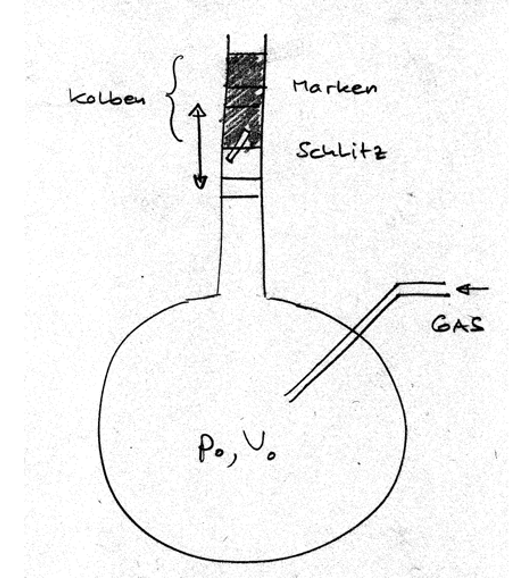
\includegraphics{skizzeIsentropenindex.png}
  \subsection{Ger\"ateliste}
  \subsubsection{Apparatur nach \itshape{Clement-Desormes}\/}
  Gro{\ss}e, isolierte Glasflasche mit Luft Ein-/Auslassventil,
  Fl\"ussigkeitsmanometer zum ablesen der Druckdifferenz zum Au{\ss}endruck. Die 
  Manometerfl\"ussigkeit ist ein \"Athanol-Wasser-Gemisch. Eine Gummiball-pumpe
  wird verwendet um den Luftdruck in der Flasche gegen\"uber dem Au\ss~endruck zu 
  erh\"ohen.
  \subsubsection{Apparatur nach \itshape{Flammersfeld}\/}
  Glaskolben mit aufgesetztem Pr\"azisions-Glaszylinder und Kunststoffkolben. Argon, 
  Stickstoff und Kohlendioxid in Stahlflaschen. Lichtschranke mit Z\"ahler. Elektronische
  Handstoppuhr (wobei wir eine Mobiltelefon-Uhr verwendet haben). Barometer.
  \section{\underline{Auswertung}}
\subsection{\underline{Aufgabe 1}}
Zur Auswertung der Messergebnisse benötigt man nach (21) die Mittelwerte von $\Delta h_{1} $ und $\Delta h_{2}$:
\begin{align*}
  <\Delta h_{1}> = 42.67 \\
  <\Delta h_{2}> = 7.33
\end{align*}
Nach (21) ergibt sich dann
\begin{align*}
  \kappa &= \frac{42.67}{42.67-7.33} = 1.21
\end{align*}
\subsubsection{Fehlerbetrachtung}
Nach Gauß'scher Fehlerfortpflanzung:
\begin{align*}
    \Delta \kappa &= \sqrt{{\left(\frac{- \Delta h_{2}}{{(\Delta h_{1}-\Delta
    h_{2})}{^2}}\right)}^{2} \cdot {(\Delta(\Delta h_{1}))}^{2}+{\left(\frac{\Delta
    h_{1}}{{(\Delta h_{1} - \Delta h_{2})}^{2}}\cdot (\Delta(\Delta h_{3}))\right)}^{2}}\\
&= 0.069
\end{align*}
Damit ergibt sich als Endwert
\begin{equation*}
  \kappa = 1.21 \pm 0.07
\end{equation*}

\subsubsection{Referenzwert Kappa}
Die theoretische Betrachtung über die Freiheitsgrade f = 5 für Luft sieht nach
(33) wie folgt aus:
\begin{align*}
    \kappa = \frac{7}{5} = 1.4
\end{align*}
\subsection{\underline{Aufgabe 2}}
 Nach (28) k\"onnen wir nun die jeweiligen Isentropenindizes von Ar, $N_{2}$ und $CO_{2}$
 bestimmen. Demnach ist 
 \begin{align*}
     {\kappa}_{Ar} &=\frac{4{\pi}^{2}\cdot0.00452\cdot1142\cdot{10}^{-6}}
     {{0.3294}^{2}\cdot99700{(\pi\cdot{0.00595}^{2})}^{2}} \approx 1.52 \\ \\
     {\kappa}_{{N}_{2}} &= \frac{4{\pi}^{2}\cdot0.00458\cdot1145\cdot{10}^{-6}}
     {{0.3515}{2}\cdot99700{(\pi\cdot{0.00595}^{2})}^{2}} \approx 1.36 \\ \\
     {\kappa}_{{CO}_{2}} &= \frac{4{\pi}^{2}\cdot0.0045\cdot1147\cdot{10}^{-6}}
     {{0.3585}^{2}\cdot99700{(\pi{0.00595}^{2})}^{2}} \approx 1.29
 \end{align*}
 \subsubsection{Fehlerbetrachtung}
 Alle Fehler ausser der von T und V k\"onnen vernachl\"assigt werden,
 da in der Fehlerfotpflanzung die werte $\Delta~m$ mit 0.00034, $\Delta~p$ mit 0.000015
 und $\Delta~S$ mit 0.0000017 ungef\"ahr in $\kappa$ eingehen, sind diese gegen\"uber
 $\Delta~T$ und $\Delta~V$ vernachl\"assigbar.
 $\Delta\kappa$ l\"asst sich nach folgender Formel berechnen:
 \begin{align*}
    \sqrt{{\left(
              \frac{4{\pi}^{2}-2mV}{{T}^{2}p{s}^{2}}\Delta~T
            \right)}^{2}+
            {\left(
              \frac{4{\pi}^{2}V}{{T}^{2}p{s}^{2}}\Delta~m
            \right)}^{2}+
            {\left(
              \frac{4{\pi}^{2}m}{{T}^{2}p{s}^{2}}\Delta~V
            \right)}^{2}+
            {\left(
              \frac{4{\pi}^{2}mV}{{T}^{2}{p}^{2}{s}^{2}}\Delta~p
            \right)}^{2}+
            {\left(
              \frac{4{\pi}^{2}mV2\pi}{{T}^{2}p{r}^{3}}\Delta~r
            \right)}^{2}
        }
 \end{align*}
 F\"ur unsere fehler erhalten wir somit:
 \begin{align*}
     \Delta{\kappa}_{Ar} &\approx 0.02 \\
     \Delta{\kappa}_{{N}_{2}} &\approx 0.02 \\ 
     \Delta{\kappa}_{{CO}_{2}} &\approx 0.02
 \end{align*}
 Also sind unsere Endergebnisse:
 \begin{align*}
     {\kappa}_{Ar} &= 1.52 \pm 0.02 \\
     {\kappa}_{{N}_{2}} &= 1.36 \pm 0.02 \\
     {\kappa}_{{CO}_{2}} &= 1.29 \pm 0.02
 \end{align*}
 \subsubsection{Theoretische Betrachtung}
Argon ist einatomig. Dementsprechend hat es 3 Freiheitsgrade. Stickstoff ist zweiatomig, hat also 5 Freiheitsgrade. Kohlenstoffdioxid hat 3 Atome, also 6 Freiheitsgrade.
\begin{align*}
  \kappa_{Ar} &= 5/3 = 1.67 \\
  \kappa_{N_{2}} &= 7/5 = 1.4 \\
  \kappa_{CO_{2}} &= 8/6 =1.33
\end{align*}
\newpage
 \section{\underline{Diskussion}}
 Die durch uns best

\newpage
 \section{\underline{Messwerte}}
 \subsection{Tabelle 1: Methode nach Clement-Desormes:}
 \begin{tabular}{Format}
     Versuch Nr. & $h_{0}$ in mm & $h_{1}$ in mm & $h_{2}$ in mm \\
     1 & 27 & 69 & 36 \\
     2 & 27 & 70 & 34 \\
     3 & 27 & 70 & 33
 \end{tabular}
 \subsection{Tabelle 2: Methode nach Flammersfeld-R\"uchart}
 \begin{tabular}{FORMAT}
     Versuch Nr. & Ar $T_{100}$ in s & $N_{2}$ $T_{100}$ in s & $CO_{2}$ $T_{100}$ in s \\
     1 & 32.9 & 36.0 & 35.6 \\
     2 & 33.0 & 35.2 & 36.4 \\
     3 & 32.9 & 35.0 & 36.0 \\
     4 & 33.0 & 35.5 & 35.6 \\
     5 & 33.0 & 35.0 & 35.6 \\
     6 & 33.1 & 34.8 & 36.0 \\
     7 & 32.7 & 34.7 & 36.1 \\
     8 & 33.1 & 35.1 & 36.0 \\
     9 & 32.8 & 35.1 & 35.6 \\
     10 & 32.9 & 35.1 & 35.6
 \end{tabular}

 \section{weiteres}
 Gemessener Luftdruck: 997mbar \plusminus~1mbar \\
 Fehler \Delta~h = \plusminus2 mm 
\end{document}
